% !TeX root = ../main.tex
% Add the above to each chapter to make compiling the PDF easier in some editors.

\chapter{Implementation}\label{chapter:implementation}
Building on the framework architecture explained in Chapter \ref{chapter:Approach}, we describe the middleware proof-of-concept (POC) implementation in details to show that the framework architecture is sound. Moreover we describe the flows implementation used to create the use cases in order tp provide the evaluation for the framework. \\

\section{Middleware}

 The middleware is written in Java, it uses \textit{Maven} as a  software project dependency management which handles the middleware build. \textit{Maven} projects contain a Project Object Model (POM) file which describes the dependencies and libraries used by the project. In addition, it has build configuration management that is used to build the project and create a runnable jar file. The middleware can be compiled and packaged to a jar using the following command \verb|mvn clean package|. The project contains dependencies for \textit{Lombok} which is a library that generates getters, setters and constructors during compile time without the need to write them in the Java classes, \textit{Gson} dependency in order to be able to read and write in JSON format, \textit{SCAMPI API} which allows us to publish, subscribe and override  functions from SCAMPI, dependencies to create a web application via \textit{Spring Boot}. \\
 
 \noindent The project is divided into several packages, we describe them in alphabetical order.
 \begin{itemize}
 
  \item First, the package \verb|com.middleware.api| which contains two classes, \verb|SCAMPApi.java|  and \verb|MiddlewareApi.java|. The class \verb|SCAMPIApi.java| has a field of type \verb|APP_LIB| from SCAMPI Java API which contains the core methods of SCAMPI server to connect, add status listeners, publish and subscribe to messages.  As shown in \ref{fig:cd-api}, \verb|SCAMPIApi| implements two classes via the \verb|APP_LIB| for the SCAMPI server which includes functions like \verb|OnConnected()|, \verb|OnDisconnected()|, \verb|OnConnectFailed()| and \verb|OnStopped()|. It also implements \verb|messageReceived()| which handles the messages once they are received from SCAMPI. Further, It contains a cache for messages and a field indicating the machine specification.
 
The class \verb|MiddlewareApi.java| contains REST API for the middleware web application that runs on port \verb|8080|. It has two requests \verb|POST /publish| and \verb|POST /subscribe|  that connect to  \verb|APPL_LIB| in order to submit publish and subscribe requests to SCAMPI server. The class \verb|MiddlewareAPI.java| has a field for the \verb|topicMapping| which is the topic-endpoint mapping we explained in \ref{subsec:usage}. Last but no least, it has a main method which in Java is used to run a class. In this case, it is used to run the built  jar file from \textit{Maven} which means once the jar file runs via the command \verb|java -jar interface-1.0-SNAPSHOT.jar|, the main method is only thing that runs and therein it starts a web application via \textit{Spring Boot}.
 \begin{figure}[H]
 	\centering
 	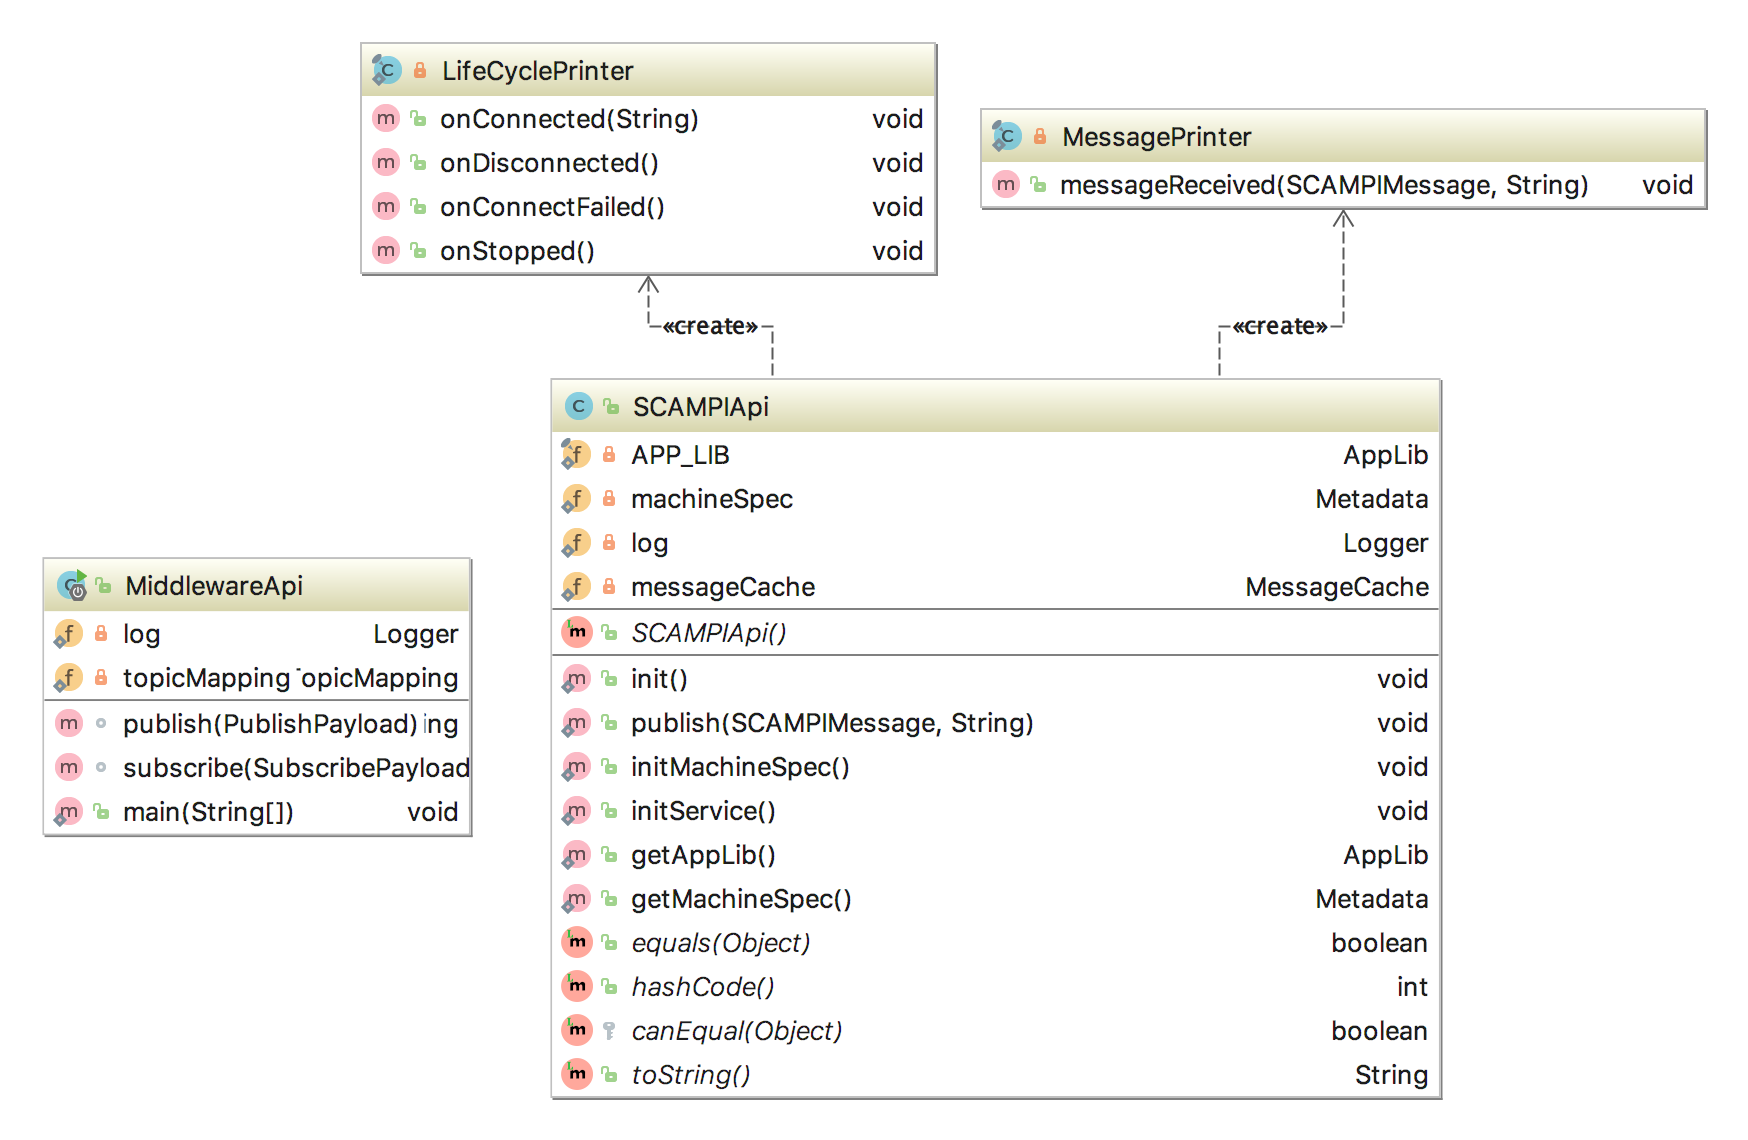
\includegraphics[scale=0.2]{images/cd-api.png}
 	\caption{Class diagram for the api package. }
 	\label{fig:cd-api}
 \end{figure}
 
\item The second package is called \verb|com.middleware.constants| and has one class \verb|Constants.java| which contains all the constant fields used in the middelware across all other classes. This includes string keys for SCAMPI messages, some Linux commands,  URL for the local node-RED instance, path for user home directory on the hosting machine and path for the JSON file that includes the machine specification. Furthermore, it contains the topic reserved for computations named \textit{Main} \\
 
 
 \item The third package is the most important one \verb|com.middleware.domain| which contains most of the services that is handled by the middleware. There are two singleton classes namely \verb|ToppicMapping.java| and \verb|MessageCache.java| that means there exist only one instance across the whole web application no matter how long it runs and no other class can create a new instance of these types. Thats because both are types of caches which should be consistent and global to any class which would need these caches. 
 
 The classes \verb|CommandRunner.java| and \verb|RESTHandler.java| are helpers. The first is used to run commands on the machine and  has two methods \verb|run(String)| and \verb|getFreeRam()| which is equivalent to calling \verb|run("free -m" )|. The second class is used as a REST client for sending requests to node-RED which are used to deploy computations and  send data to endpoints.
 
  Next are the classes \verb|MessageHandler.java| and \verb|Publisher.java| which contain the services for handling incoming messages from SCAMPI and publishing new message respectively. The \verb|MessageHandler.java| is called from  \verb|SCAMPIApi.java| method \verb|messageRecieved()| and differentiates between two types of the messages; computation ones which are received on the topic \textit{Main} and handles them with the method \verb|handleMainTopic(SCAMPIMessage)| which takes care of the resources, machine specifications, puts dependencies on node-RED local directory then the \verb|RESTHandler.java| class is used to deploy the computation to node-RED, and data messages which are received on other topics and handles them with the method \verb|handleSpecialTopic(ScampiMessage)|, it sends the data to any subscribed endpoint in the \verb|toppicMapping| cache using also the \verb|RESTHandler.java|.
 
 The \verb|Pubisher| is responsible for submitting publish requests to the \verb|APP_LIB|. It is called from the \verb|MiddlewareApi.java|.  It creates a unique identifier for each new message, and adds the publisher global identifier to the \textit{SCAMPIMessage} as well. It has the same topic differentiation as \verb|MessageHandler.java|.
 On the one hand, if the publish topic is \textit{Main}, it collects the dependencies and attach it to the \textit{SCAMPIMessage} before it sends the message to SCMAPI server. On the other hand, if it is a data topic it checks the attachments and adjusts the response endpoint  to whether it should be sent back to this node only, if this is the case, it creates a mapping between the global identifier of the node and the endpoint that sent the publish request then send it to SCAMPI server. \\
 
 \begin{figure}[H]
 	\centering
 	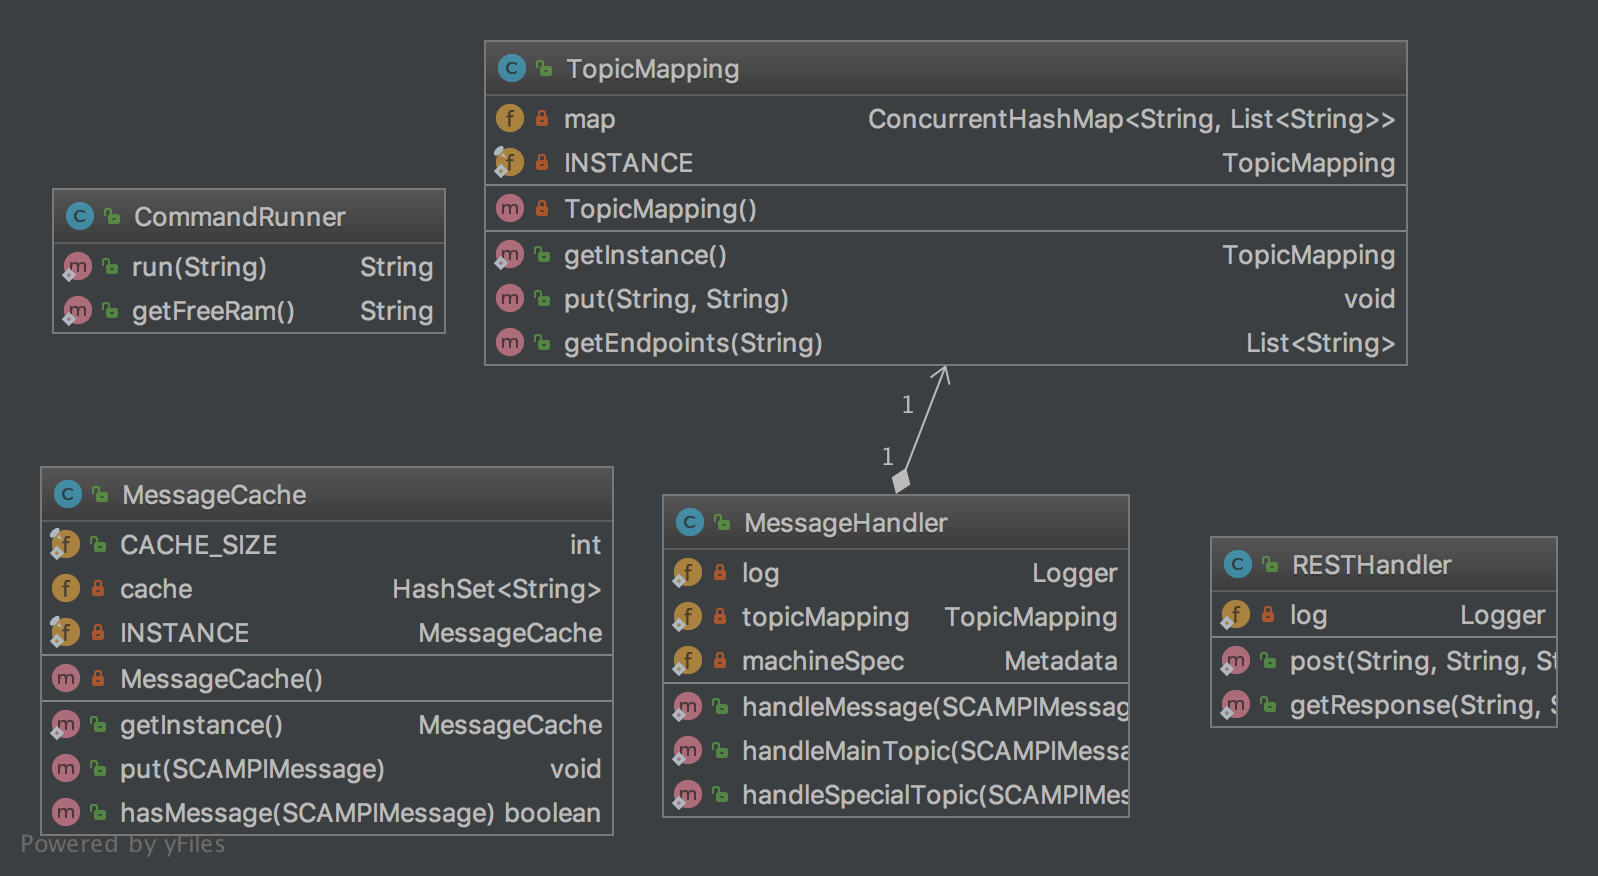
\includegraphics[scale=0.25]{images/cd-domain.png}
 	\caption{Class diagram for the domain package. }
 	\label{fig:cd-domain}
 \end{figure}


\item The fourth package \verb|com.middleware.exception| which contains the project's custom exceptions. Currently it only has a \verb|RESTFailedException.java| class which handles node-RED deployments and data requests failures.

\item The fifth and last package is \verb|com.middleware.model|, it holds the models which are classes used to hold data and encapsulate them. Note that the Java classes do not contain any getters and setters or constructors. However, using \textit{Lombok} library they are generated in compile time and they can be picked up by the Integrated Development Environment (IDE) as shown in \ref{fig:cd-models}. 

 \begin{figure}[H]
	\centering
	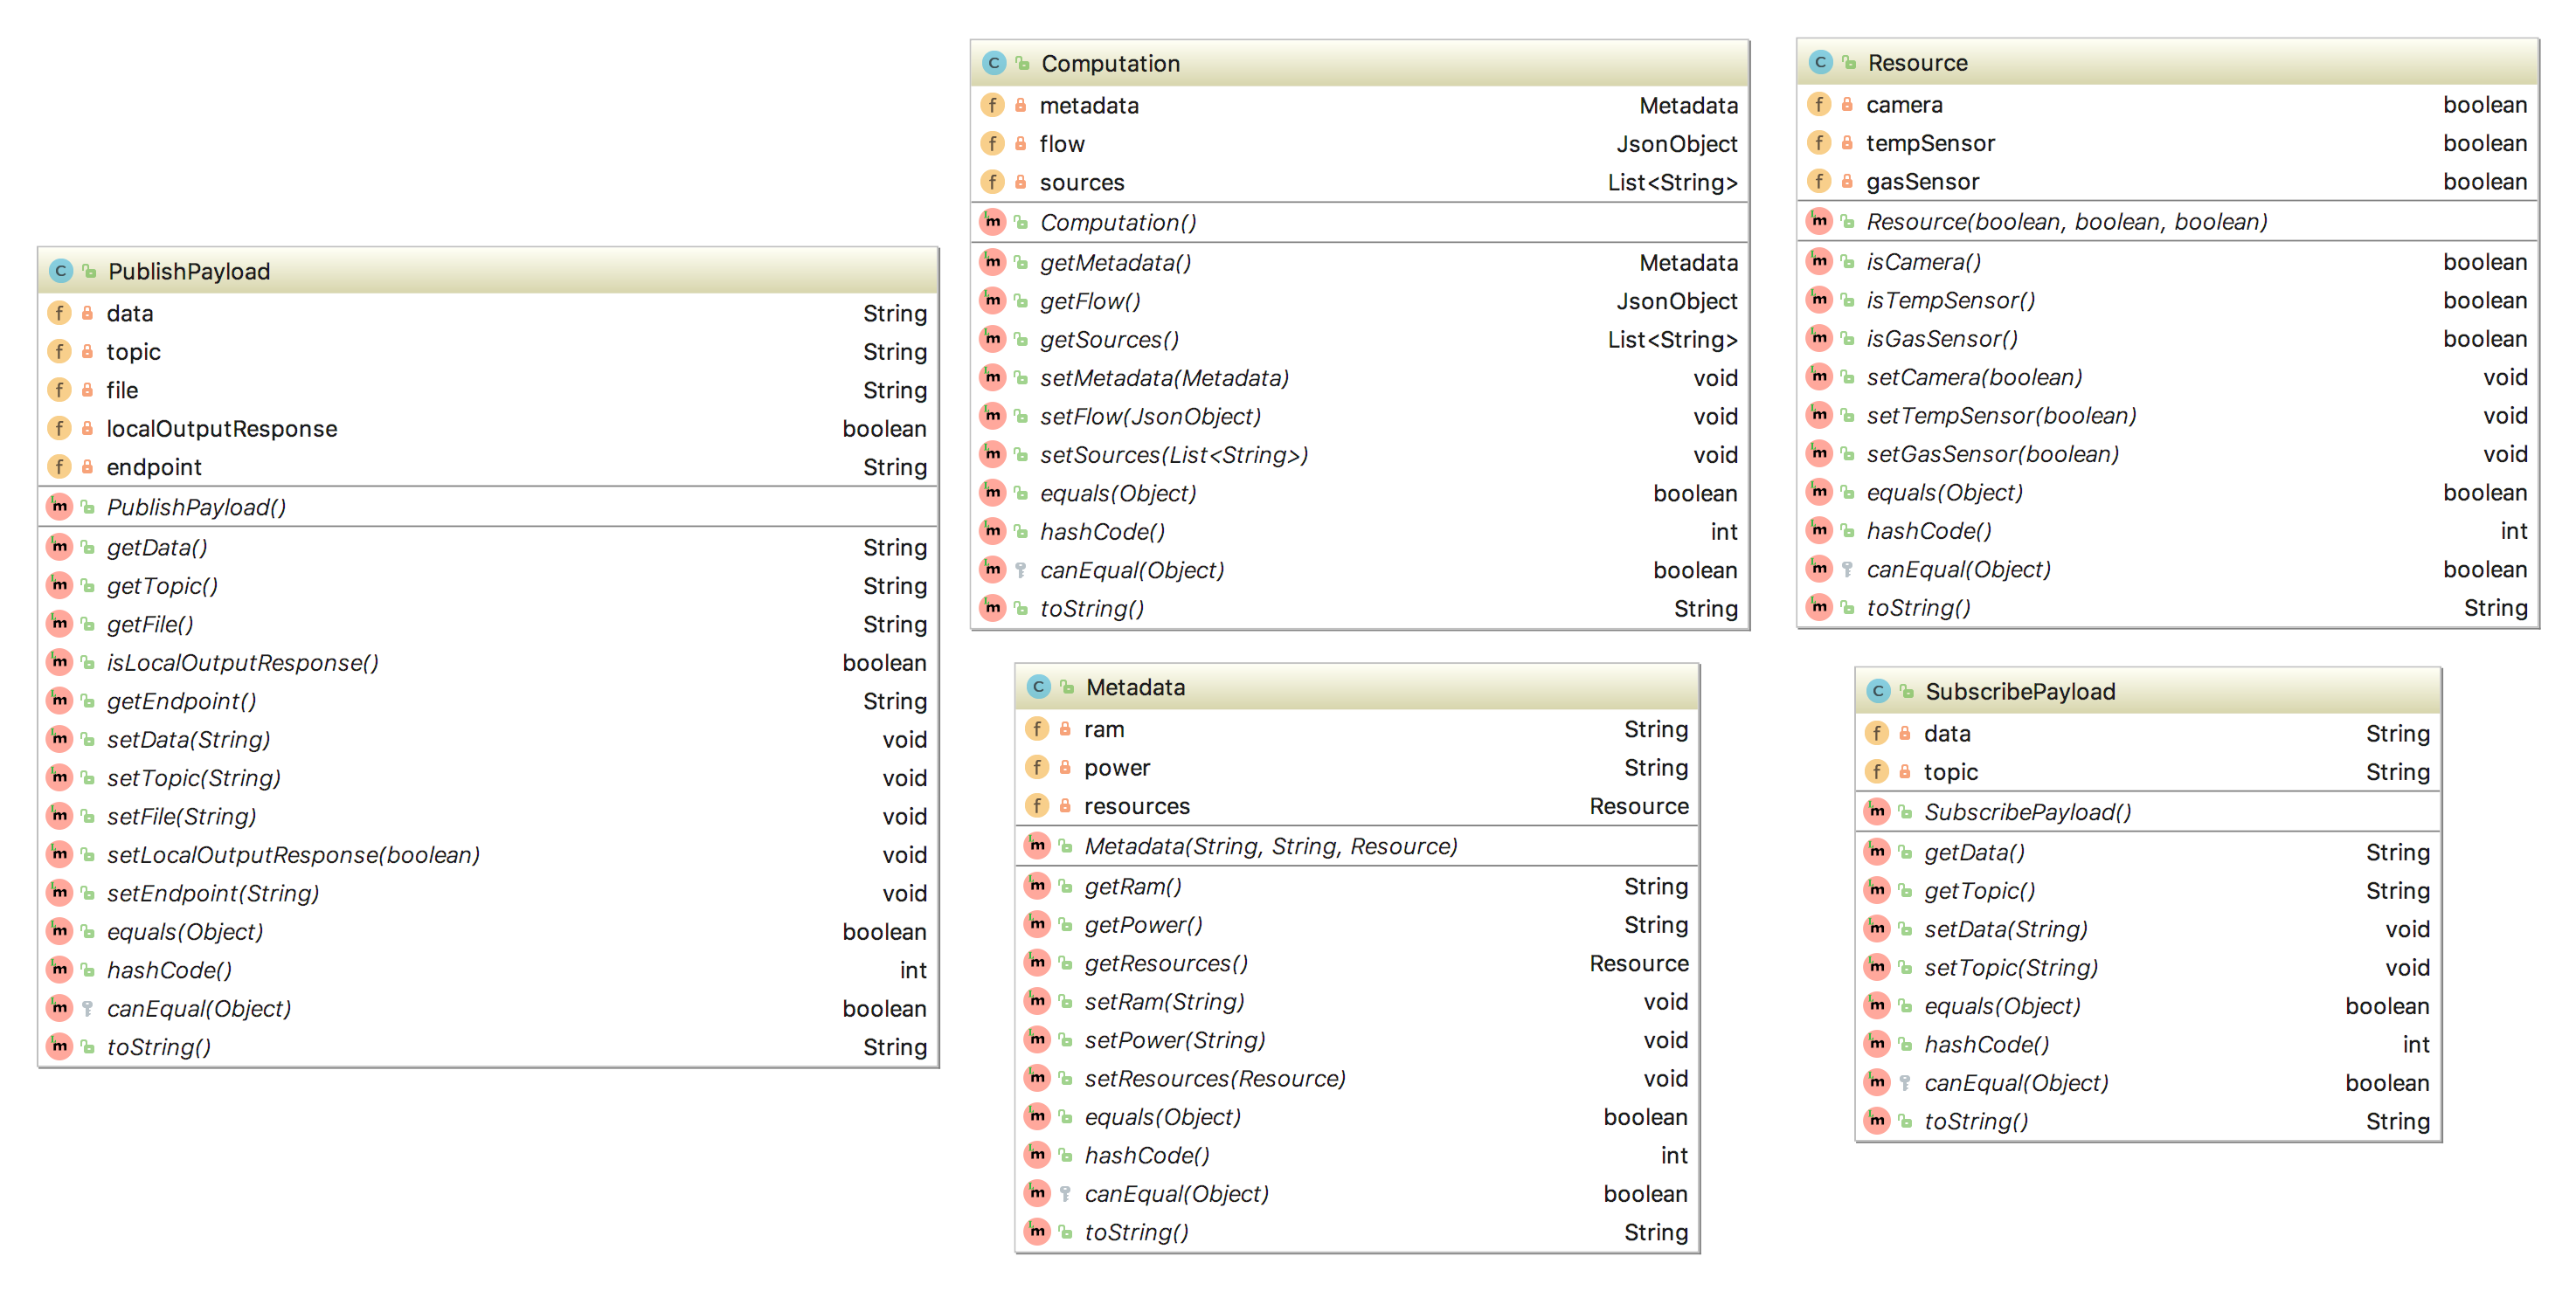
\includegraphics[scale=0.13]{images/cd-models.png}
	\caption{Class diagram for the model package. }
	\label{fig:cd-models}
\end{figure}

\end{itemize}


\section{Flows}
This section explains all the flows developed in this thesis. It shows how the flows can be implemented to achieve different use cases. It also shows how we use node-RED flows in order to send computations.
\subsection{Send Computations}
In order to deliver flows which expresses computations for all nodes or selected ones according to available resources,  sensors, actuators and also attach dependencies, we developed a node-RED flow shown in figure \ref{fig:flow-publish-computation}. The flow responds to the endpoint \verb|GET localhost:1880/publish| and returns the HTML page in figure \ref{fig:html-publish}. Afterwards, the user can adjust the computation power needed by the flow, necessary free Random Access Memory(RAM), sensors and actuators. Then he/she must also write the flow identifier and attach dependencies, and eventually click on the button \textit{push}, which calls another endpoint on the same flow \verb|localhost:1880/push|, it receives the data, fetches the flow details and publish it to the middleware which handles the rest.
 \begin{figure}[H]
	\centering
	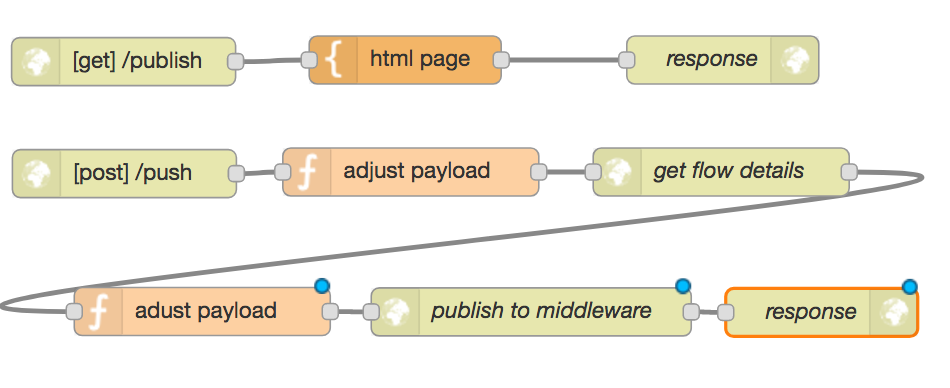
\includegraphics[scale=0.6]{images/flow-publish-computation.png}
	\caption{A flow that publishes computations to the middleware dn thus to SCAMPI.}
	\label{fig:flow-publish-computation}
%\end{figure}
 %\begin{figure}[H]
	\centering
	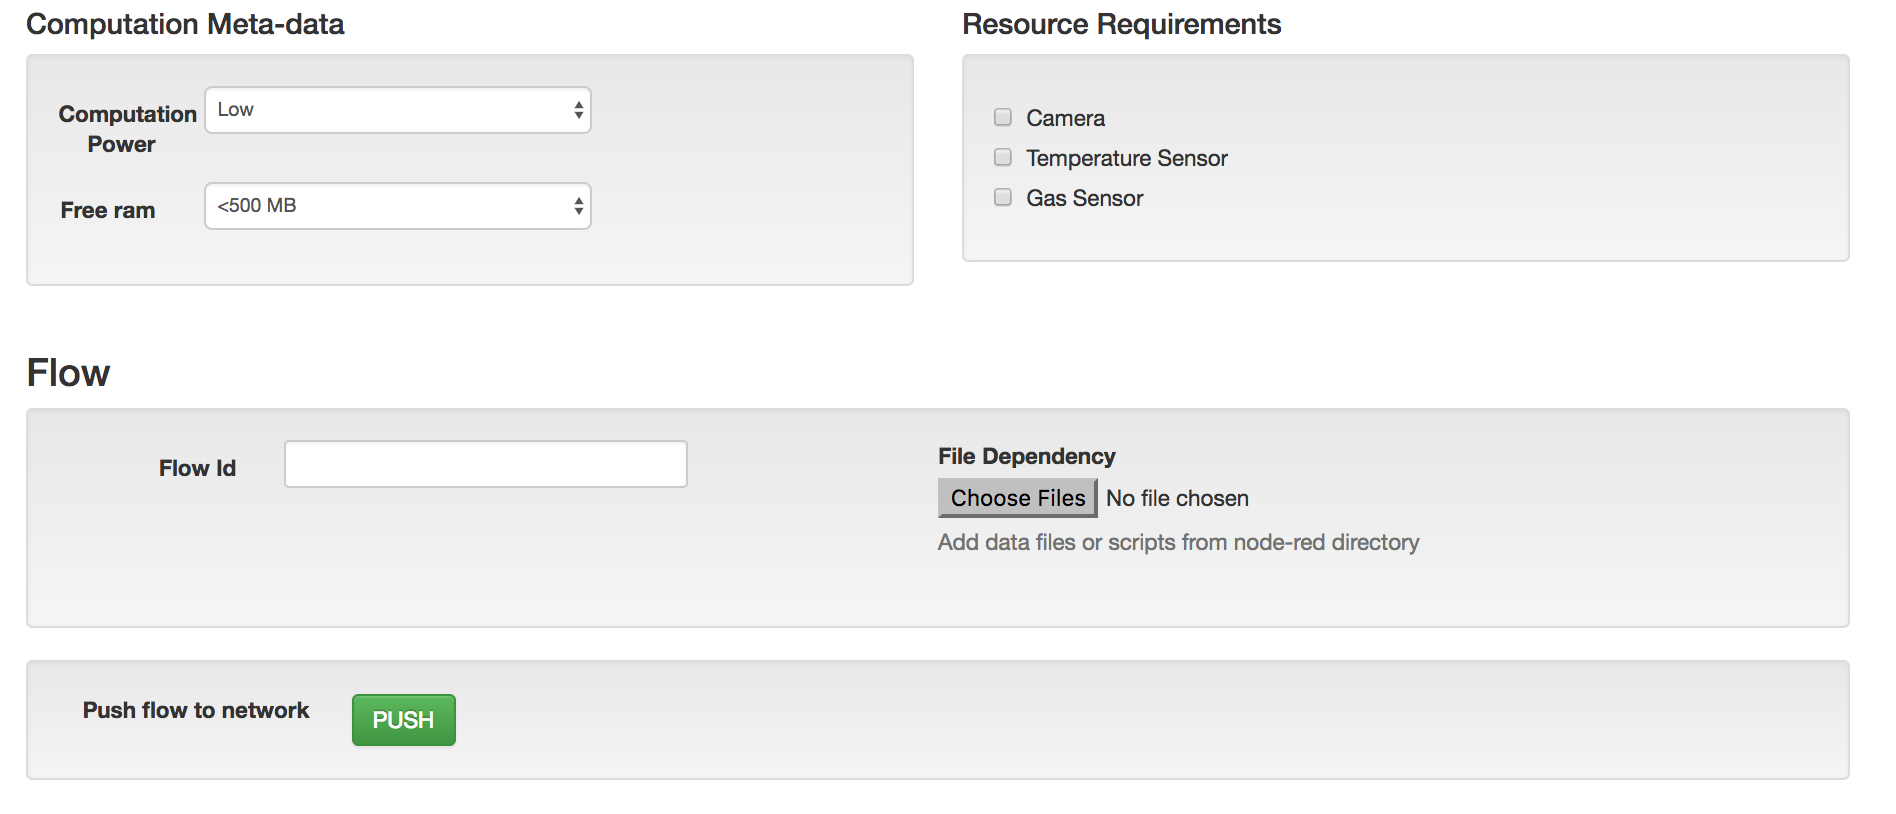
\includegraphics[scale=0.4]{images/html-publish.png}
	\caption{The HTML page used to publish computations conveyed in \textit{html template} element.}
	\label{fig:html-publish}
\end{figure}


\subsection{Temperature Sensor Alert}
This flow was developed to make sure that the software framework works against the basic IoT usage of sensors, actuators and time-series databases. As presented in figure \ref{fig:flow-temp}, the flow runs once it was deployed to any node. Note that it would not have been deployed by the middleware without checking that it has the required resources and dependencies. Once the flow is deployed, it starts a script for sensing temperature  which is sent as a dependency while sending the flow to other nodes. It then checks if the temperature is a valid number, then it gets stored in a database. Further, if the temperature is above 30 degree Celsius it runs a script, which is also sent as a dependency, to light a red led lamp. On top of that, the flow responds to the endpoint \verb|localhost:1880/temp| and returns all the collected temperature data in the last two minutes.
 \begin{figure}[H]
	\centering
	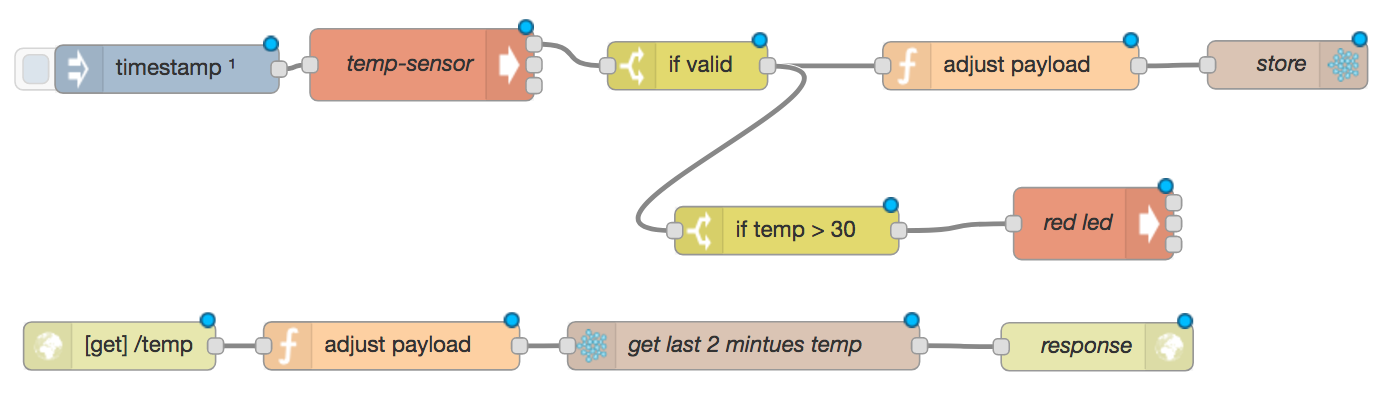
\includegraphics[scale=0.6]{images/flow-temp.png}
	\caption{A flow that reads temperature and stores it, also start a red lamp if temperature is above 30 degree Celsius.}
	\label{fig:flow-temp}
\end{figure}



\subsection{Detect Movement and Store Image Responses} \label{subsec:detect-move}
As part of the implementation evaluation, we developed this flow to take part in a bigger use case. The flow is designed to detect movement through the infrared sensor and then take a picture, which is then published on the topic \textit{NUC} for image recognition. However, in the push payload along with the picture, there is a field stating that the response should come back to this exact node, therefore, the middleware creates a mapping between the device global identifier and the endpoint before publishing. Also, as demonstrated in \ref{fig:flow-motion}, the flow awaits messages on its endpoint and executes a script which starts a red led, it also store the recognized image in a database along with its accompanying data. 

\begin{figure}[H]
	\centering
	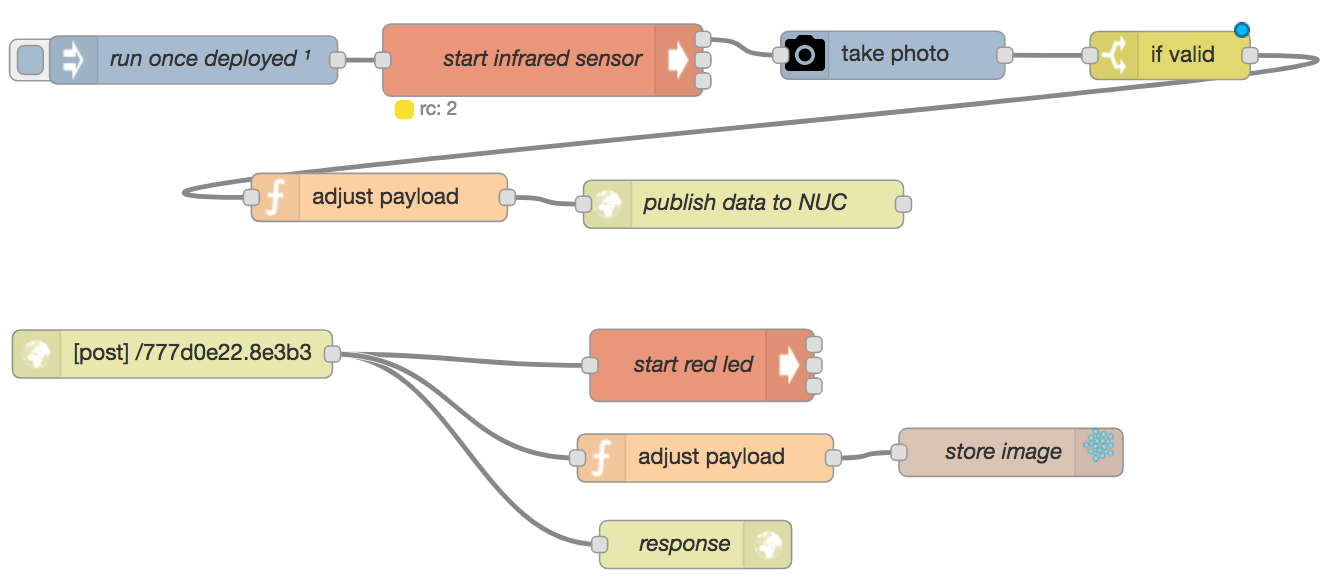
\includegraphics[scale=0.6]{images/flow-motion.png}
	\caption{A flow that detects motion, take an image, publish message and store response.}
	\label{fig:flow-motion}
\end{figure}


\subsection{Show Recognized images}
Since compatibility is an important part to validate in our framework. We created a simple flow to show local composable flows. It simply queries the database for recognized images from the previous flow \ref{subsec:detect-move} when requested on the endpoint \verb|GET localhost:1880/images|. It has an HTML page response showing all the images along with their image recognition confidence percentage data and time-stamp.

\begin{figure}[H]
	\centering
	
\includegraphics[scale=0.6]{images/flow-images.png}
	\caption{A flow that creates an endpoint for stored database images.}
	\label{fig:flow-image}
\end{figure}

\subsection{TensorFlow Water Bottle Recognition}
To prove that we can send flows to machines with heavy computation power and lots of free RAM. We developed an image recognition flow using \textit{TensorFlow} which is an open-source software library for machine intelligence. \textit{TensorFlow} needs a 54MB image recognition model that recognizes 1000 object classes, one of them is a water bottle. It also needs the code to run the recognition algorithm which is a Java jar file of 17.3MB size. Therefore, the flow  needs to carry all the mentioned dependencies. As show figure \ref{fig:flow-tensor}, the flow subscribes to the topic \textit{NUC} once it is deployed. Then, when the middleware that runs on the same machine receives a message on the topic \textit{NUC}, the middleware sends it to the corresponding endpoint  from the topic-endpoint mapping, it also puts the dependencies in node-RED directory. Thereafter, the flow uses the message payload which should be an image, and runs the jar. If it results in a water bottle as a best match, the flow responds to the sender with the result and a confidence percentage.
 \begin{figure}[H]
	\centering
	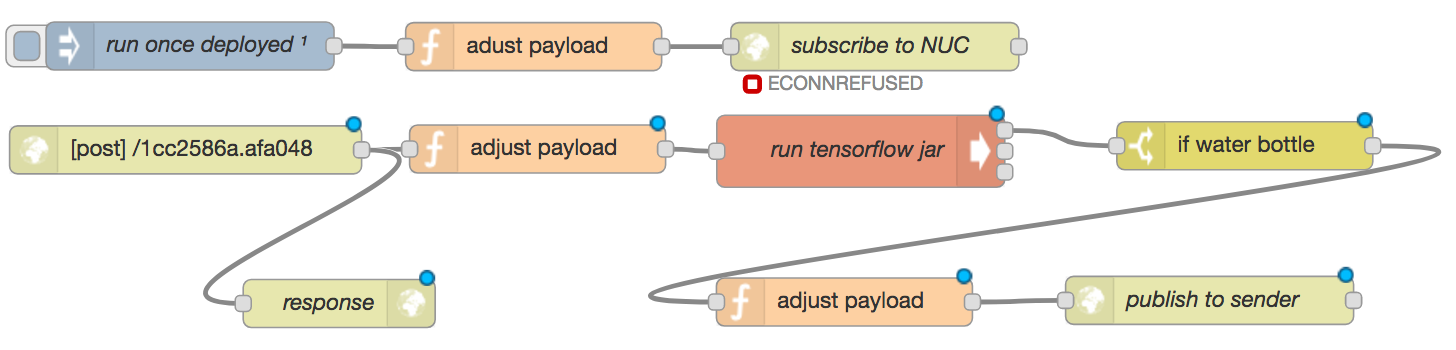
\includegraphics[scale=0.6]{images/flow-tensor.png}
	\caption{A flow that uses tensorflow to recognize a water bottle.}
	\label{fig:flow-tensor}
\end{figure} 
